\chapter{Bayesian Inference}

\begin{ex}
  Let $f$ and $g$ be PDFs of normal distributions with means $\mu_f$ and $\mu_g$
  and variances $\sigma_f^2$ and $\sigma_g^2$ respectively. Note that since
  \begin{align*}
    \frac{(x-\mu_f)^2}{\sigma_f^2}
    +\frac{(x-\mu_g)^2}{\sigma_g^2}
     & =\frac{\sigma_g^2(x^2-2x\mu_f+\mu_f^2)+\sigma_f^2(x^2-2x\mu_g+\mu_g^2)}{\sigma_f^2\sigma_g^2}                                                                                                      \\
     & =\frac{(\sigma_f^2+\sigma_g^2)x^2-2(\sigma_g^2\mu_f+\sigma_f^2\mu_g) x+\sigma_g^2\mu_f^2+\sigma_f^2\mu_g^2}{\sigma_f^2\sigma_g^2}                                                                  \\
     & =\frac{x^2-2\frac{\sigma_g^2\mu_f+\sigma_f^2\mu_g}{\sigma_f^2+\sigma_g^2} x+\frac{\sigma_g^2\mu_f^2+\sigma_f^2\mu_g^2}{\sigma_f^2+\sigma_g^2}}{\frac{\sigma_f^2\sigma_g^2}{\sigma_f^2+\sigma_g^2}} \\
     & =\frac{\left(x-\frac{\sigma_g^2\mu_f+\sigma_f^2\mu_g}{\sigma_f^2+\sigma_g^2}\right)^2}{\frac{\sigma_f^2\sigma_g^2}{\sigma_f^2+\sigma_g^2}} +C,
  \end{align*}
  for some $C$ not depending on $x$, we have
  \begin{align*}
    f(x)g(x)
     & \propto \exp\left\{-\frac{(x-\mu_f)^2}{2\sigma_f^2}\right\}
    \exp\left\{-\frac{(x-\mu_g)^2}{2\sigma_g^2}\right\}                                                                                                                                  \\
     & \propto \exp\left\{-\frac{1}{2}\frac{\left(x-\frac{\sigma_g^2\mu_f+\sigma_f^2\mu_g}{\sigma_f^2+\sigma_g^2}\right)^2}{\frac{\sigma_f^2\sigma_g^2}{\sigma_f^2+\sigma_g^2}}\right\},
  \end{align*}
  which, by inspection, is proportional to the PDF of a normal distribution with
  mean
  \[
    \frac{\sigma_g^2\mu_f+\sigma_f^2\mu_g}{\sigma_f^2+\sigma_g^2}
  \]
  and variance
  \[
    \frac{\sigma_f^2\sigma_g^2}{\sigma_f^2+\sigma_g^2}.
  \]

  Consider the product of $n$ normal PDFs each with mean $X_i$ and variance
  $\sigma^2$. Since we can group it as the product of the first $n-1$ PDFs and
  the last PDF, and since by the previous argument, the product of two normal
  PDFs is proportional to a normal PDF, it follows by induction that so is the
  product of $n$ PDFs. It only remains to figure out the mean and variance.
  Note that for $n=2$ we have
  \[
    \sigma_2^2
    =\frac{\sigma^2\sigma^2}{\sigma^2+\sigma^2}=\frac{\sigma^2}{2}
    \text{ and }
    \mu_2
    =\frac{X_1\sigma^2+X_2\sigma^2}{\sigma^2+\sigma^2}
    =\frac{X_1+X_2}{2}
    =\Xbar_2.
  \]
  Suppose that for $n-1$ we have
  \[
    \sigma_{n-1}^2=\frac{\sigma^2}{n-1}
    \text{ and }
    \mu_{n-1}=\Xbar_{n-1},
  \]
  and note that then
  \[
    \sigma_n^2
    =\frac{\sigma_{n-1}^2\sigma^2}{\sigma_{n-1}^2+\sigma^2}
    =\frac{\frac{\sigma^2}{n-1}\sigma^2}{\frac{\sigma^2}{n-1}+\sigma^2}
    =\frac{\sigma^4}{n-1} / \frac{n\sigma^2}{n-1}
    =\frac{\sigma^2}{n}
    =\se^2,\text{ and }
  \]
  \[
    \mu_n
    =\frac{\Xbar_{n-1}\sigma^2+X_n\sigma_{n-1}^2}{\sigma_{n-1}^2+\sigma^2}
    =\frac{\Xbar_{n-1}\sigma^2+X_n\frac{\sigma^2}{n-1}}{\frac{\sigma^2}{n-1}+\sigma^2}
    =\frac{(\sum_{i=1}^n X_i)\sigma^2}{n-1}/\frac{n\sigma^2}{n-1}
    =\Xbar_n.
  \]
  The result follows by induction.

  Next, consider the product of $n$ normal PDFs with mean $X_i$ and
  variance $\sigma^2$ respectively, and a normal PDF with mean $a$ and variance
  $b^2$. The product of the first $n$ PDFs is proportional to an
  $N(\Xbar, \se^2)$ PDF, and therefore the full product is
  proportional to an $N(\overline{\theta}, \tau^2)$ PDF, where
  \[
    \tau^2=\frac{\se^2b^2}{\se^2+b^2},\text{ and}
  \]
  \begin{align*}
    \overline{\theta}
     & =\frac{\Xbar b^2+a \se^2}{\se^2+b^2}                        \\
     & =\frac{\Xbar b^2}{\se^2+b^2}+\frac{a \se^2}{\se^2+b^2}      \\
     & =\Xbar\frac{\frac{1}{\se^2}}{\frac{1}{\se^2}+\frac{1}{b^2}}
    +a\frac{\frac{1}{b^2}}{\frac{1}{\se^2}+\frac{1}{b^2}}          \\
     & =\Xbar\frac{\frac{1}{\se^2}}{\frac{1}{\se^2}+\frac{1}{b^2}}
    +a\left[1-\frac{\frac{1}{\se^2}}{\frac{1}{\se^2}+\frac{1}{b^2}}\right].
  \end{align*}

  Finally, let $X_1,\ldots,X_n\sim N(\theta,\sigma^2)$, where $\sigma^2$ is
  known. We take a prior $\theta\sim N(a, b^2)$, and compute the
  posterior for $\theta$. Note that
  \[
    f(\theta\,|\, X^n)
    \propto \L(\theta\,|\, X^n)f(\theta)
    = f(\theta)\prod_{i=1}^n\L(\theta\,|\, X_i)
    = f(\theta)\prod_{i=1}^n f_i(\theta),
  \]
  where $f_i$ is the PDF for an $N(X_i,\sigma^2)$ distribution. However, this is
  precisely the setting of our last proposition and therefore the result
  follows.
\end{ex}

\begin{ex}~
  \inputminted{python}{../code/11-02.py}
  \inputminted{text}{../output/11-02.txt}

  \begin{enumerate}[(a)]
    \item[(b)] Let $f(\mu)=1$. Recall that the posterior is proportional to the
          product of the likelihood and the prior and that we therefore have
          \begin{align*}
            f(\mu\,|\,x^n)\propto \prod_{i=1}^n\frac{1}{\sqrt{2\pi}}
            \exp\left\{-\frac{(x_i-\mu)^2}{2}\right\},
          \end{align*}
          and therefore, by comparison to the probability density function of a
          multivariate normal distribution,
          \begin{align*}
            f(\mu\,|\,x^n)=
            (2\pi)^{-n/2}
            \exp\left\{-\frac{\sum_{i=1}^n(x_i-\mu)^2}{2}\right\}.
          \end{align*}

          \begin{figure}[H]
            \centering
            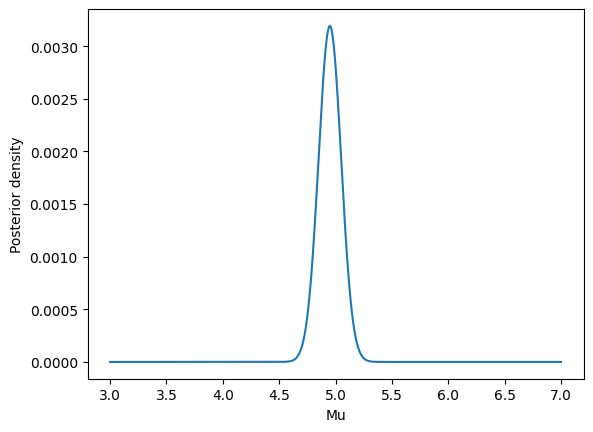
\includegraphics[scale=0.8]{../images/11-02b}
            \caption{Plot of the posterior density of $\mu$.}
          \end{figure}
    \item[(c)]~
          \begin{figure}[H]
            \centering
            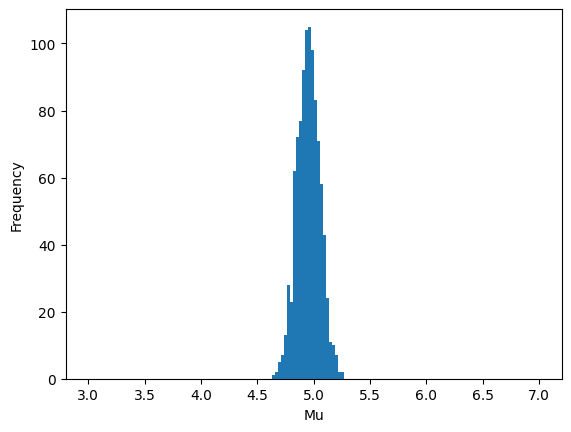
\includegraphics[scale=0.8]{../images/11-02c}
            \caption{Histogram of $1000$ simulated values drawn from the
              posterior density of $\mu$.}
          \end{figure}
    \item[(d)] Let $\theta=e^\mu$. We then have
          \begin{align*}
            \P{\Theta\leq \theta\,|\,x^n}
             & =\P{e^\mu\leq \theta\,|\,x^n}                            \\
             & =\P{\mu\leq \log{\theta}\,|\,x^n}                        \\
             & =\int_{-\infty}^{\log{\theta}}\!f(\mu\,|\,x^n)\,\d{\mu},
          \end{align*}
          and therefore, by differentiating under the integral sign,
          \[
            f(\theta\,|\,x^n)
            =\frac{\d}{\d\theta}\P{\Theta\leq \theta\,|\,x^n}
            =\frac{1}{\theta}(2\pi)^{-n/2}
            \exp\left\{-\frac{\sum_{i=1}^n(x_i-\log{\theta})^2}{2}\right\}.
          \]
          \begin{figure}[H]
            \centering
            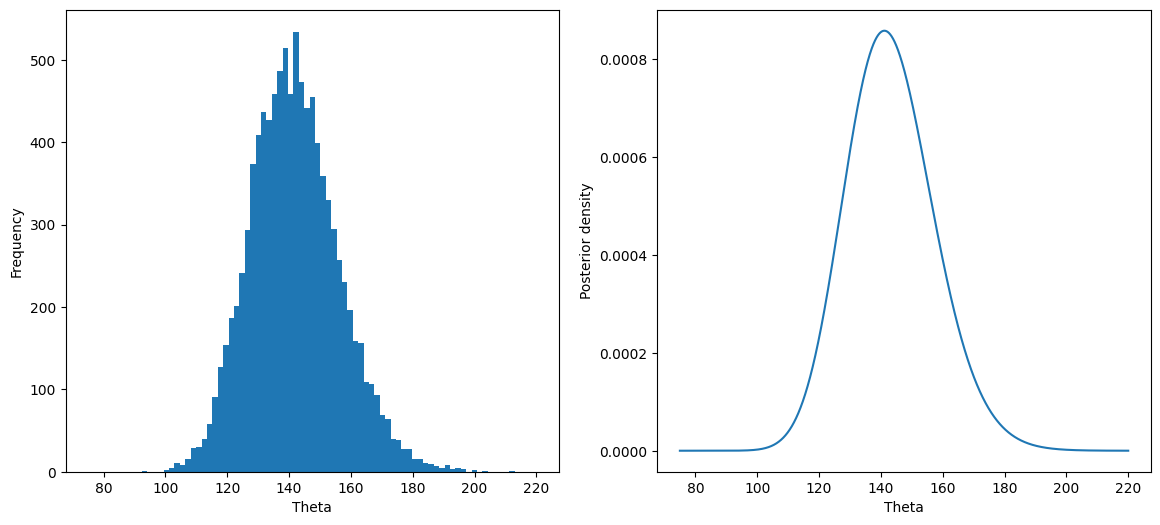
\includegraphics[scale=0.54]{../images/11-02d}
            \caption{A histogram of $10,000$ simulated values of $\theta$ drawn
              using the posterior density of $\mu$ (left) and a plot of the
              exact analytically computed posterior distribution of $\theta$
              (right).}
          \end{figure}
    \item[(e)] As per the output of the code giving in the listing at the start
          of this problem, a 95\% posterior interval for $\mu$ is given by
          $[4.754, 5.146]$.
    \item[(f)] From the output of the code listing at the top, a 95\%
          posterior interval for $\theta$ is given by $[116.004, 171.681]$. Note
          that we are asked for a confidence interval, but per Theorem
          11.5 we may approximate it with a Bayesian posterior interval instead.
  \end{enumerate}
\end{ex}

\begin{ex}
  Note that
  \[
    \L(\theta, x_i)=\begin{cases}
      0          & \theta < x_i,     \\
      x_i/\theta & \text{otherwise},
    \end{cases}
  \]
  and that therefore
  \[
    \L(\theta, x^n)=\begin{cases}
      0                                  & \theta < x_{(n)}, \\
      \frac{\prod_{i=1}^n x_i}{\theta^n} & \text{otherwise}.
    \end{cases}
  \]
  Thus, if $f(\theta)\propto 1/\theta$,
  \[
    f(\theta\,|\, x^n)\propto \begin{cases}
      0                                      & \theta < x_{(n)}, \\
      \frac{\prod_{i=1}^n x_i}{\theta^{n+1}} & \text{otherwise},
    \end{cases}
  \]
  or, since
  \[
    \int_{x_{(n)}}^\infty \frac{\prod_{i=1}^n x_i}{\theta^{n+1}}\,\d\theta
    =\frac{1}{n}\prod_{i=1}^n\frac{x_i}{x_{(n)}},
  \]
  \[
    f(\theta\,|\, x^n)=\frac{n(x_{(n)})^n}{\theta^{n+1}}I_{[x_{(n)},\infty)}(\theta).
  \]
\end{ex}

\begin{ex}~
  \begin{enumerate}[(a)]
    \inputminted{python}{../code/11-04.py}
    \inputminted{text}{../output/11-04.txt}
    \item By Exercise 9.7, the MLE for $\tau$ is given by
          \[
            \tauhat = \phat_1 -\phat_2=X_1/n_1-X_2/n_2,
          \]
          with
          \[
            \sehat=\sqrt{
              \frac{\phat_1(1-\phat_1)}{n_1}
              +\frac{\phat_2(1-\phat_2)}{n_2}.
            }
          \]
          In particular, we have that the MLE for $\tau$ is $0.2$. The estimated
          standard error is $0.08944$, and a 90\% confidence interval
          is given by $[0.05288, 0.3471]$.
    \item From the code listing given at the start of the problem, we can see
          that a 90\% confidence interval for $\tau$ using the parametric
          bootstrap method is given by $[0.06, 0.34]$.
    \item Using the prior $f(p_1,p_2)=1$, it follows that the posterior mean of
          $\tau$ is $0.1953$, and a 90\% posterior confidence interval is given
          by $[0.04632, 0.3393]$.
    \item Let
          \[
            \psi=g(p_1,p_2)=\log\left(
            \left(\frac{p_1}{1-p_1}\right)\div
            \left(\frac{p_2}{1-p_2}\right)
            \right),
          \]
          and note that then
          \begin{align*}
            \nabla g=\begin{pmatrix}
              \frac{1}{p_1-p_1^2} \\
              \frac{1}{p_2^2-p_2}
            \end{pmatrix}.
          \end{align*}
          By the equivariance of the MLE, $\psihat=g(\phat_1,\phat_2)$, and by
          the multiparameter delta method
          \begin{align*}
            \sehat(\psihat)
             & =\sqrt{
              \begin{pmatrix}
                \frac{1}{\phat_1-\phat_1^2} &
                \frac{1}{\phat_2^2-\phat_2}
              \end{pmatrix}
              \begin{pmatrix}
                \frac{\phat_1(1-\phat_1)}{n_1} & 0                              \\
                0                              & \frac{\phat_2(1-\phat_2)}{n_2}
              \end{pmatrix}
              \begin{pmatrix}
                \frac{1}{\phat_1-\phat_1^2} \\
                \frac{1}{\phat_2^2-\phat_2}
              \end{pmatrix}
            }
            =\sqrt{
              \frac{1}{n_1(\phat_1-\phat_1^2)}+
              \frac{1}{n_2(\phat_2^2-\phat_2)}
            }.
          \end{align*}
          In particular, we have that the MLE of $\psi$ is $0.9808$. The
          estimated standard error is $0.2041$, and a 90\% confidence interval
          for $\psi$ is given by $[0.6451, 1.317]$.
    \item Under the prior $f(p_1,p_2)=1$, the posterior mean of $\psi$ is
          $0.9693$, a 90\% posterior confidence interval is given by
          $[0.2244, 1.737]$.
  \end{enumerate}
\end{ex}

% 5
\begin{ex}~
  \inputminted{python}{../code/11-05.py}
  \begin{figure}[H]
    \centering
    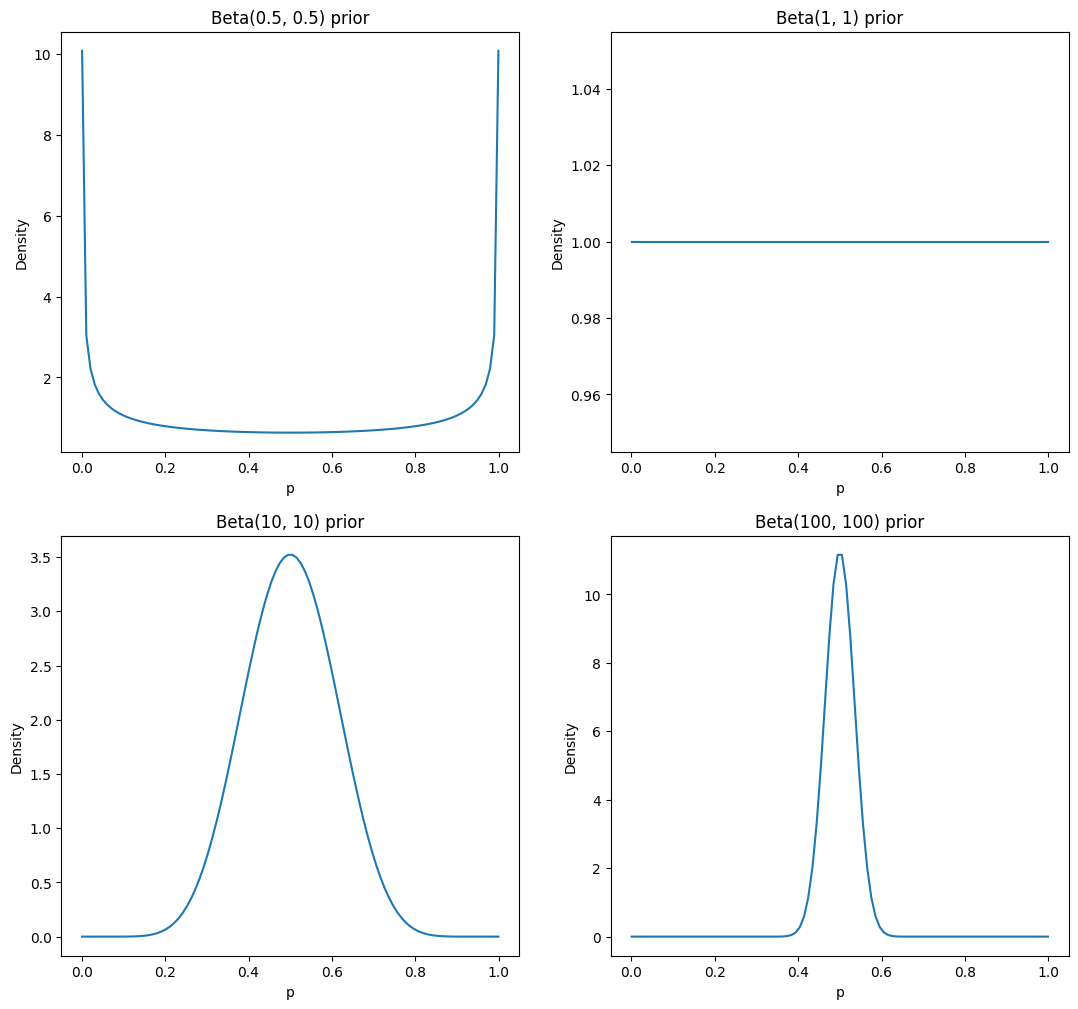
\includegraphics[scale=0.57]{../images/11-05a}
    \caption{
      Plots of the prior distributions of $p$ given by
      $\text{Beta}(\alpha, \alpha)$ distributions for different values of
      $\alpha$. Note that in all cases, the distribution is centered at $1/2$,
      but becomes more sharply peaked as $\alpha$ increases.
    }
  \end{figure}
  \begin{figure}[H]
    \centering
    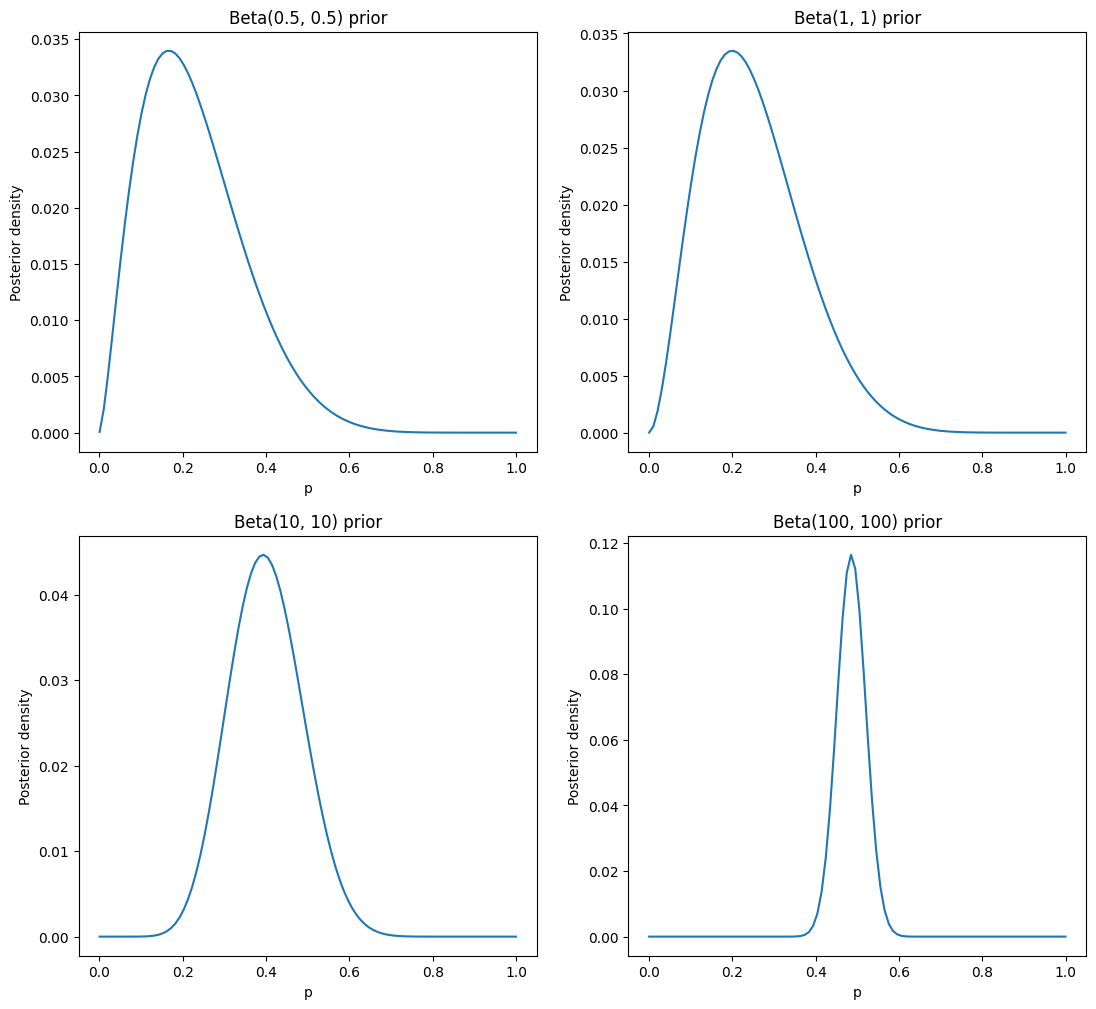
\includegraphics[scale=0.57]{../images/11-05b}
    \caption{
      Plots of the different posterior distributions for $p$ given the prior
      distributions from the previous figure. Note that the larger $\alpha$ is,
      the less sensitive the posterior is to the data.
    }
  \end{figure}
\end{ex}

\begin{ex}
  Let $X_1,\ldots,X_n\sim\text{Poisson}(\lambda)$.
  \begin{enumerate}[(a)]
    \item Recall that if $\lambda\sim\text{Gamma}(\alpha,\beta)$,
          \[
            f(\lambda)=\frac{1}{\beta^\alpha\Gamma(\alpha)}\lambda^{\alpha-1}e^{-\lambda/\beta},
          \]
          and that therefore
          \begin{align*}
            f(\lambda\,|\,x^n)
             & \propto \left(\prod_{i=1}^n e^{-\lambda}\frac{\lambda^{x_i}}{x_i!}\right)
            \frac{1}{\beta^\alpha\Gamma(\alpha)}\lambda^{\alpha-1}e^{-\lambda/\beta}     \\
             & \propto \lambda^{\alpha-1+\sum_{i=1}^nx_i}e^{-\lambda(\beta n+1)/\beta},
          \end{align*}
          and hence
          \[
            f(\lambda\,|\,x^n)
            =\frac{1}{\beta'^{\alpha'}\Gamma(\alpha')}\lambda^{\alpha'-1}e^{-\lambda/\beta'},
          \]
          where
          \[
            \alpha'=\alpha+\sum_{i=1}^nx_i,\text{ and }
            \beta'=\frac{\beta}{n\beta +1}.
          \]
          Note that the mean of a $\text{Gamma}(\alpha', \beta')$ distribution
          is at $\alpha'\beta$, and that therefore the posterior mean is
          \[
            \left(\alpha+\sum_{i=1}^nx_i\right)
            \left(\frac{\beta}{n\beta +1}\right).
          \]
    \item Recall that for a $\text{Poisson}(\lambda)$ distribution,
          \[
            \ell_n(\lambda)=\sum_{i=1}^n-\lambda+x_i\log(\lambda)+\log(x_i!),
          \]
          and therefore
          \[
            \frac{\d\ell_n(\lambda)}{\d\lambda}
            =\sum_{i=1}^n-1+x_i/\lambda,
            \text{ and  }
            \frac{\d^2\ell_n(\lambda)}{\d\lambda^2}
            =-\sum_{i=1}^n x_i/\lambda^2.
          \]
          Therefore, $I(\lambda)=n/\lambda$, and the Jeffreys' prior
          $f(\lambda)\propto 1/\sqrt{\lambda}$. Hence,
          \begin{align*}
            f(\lambda\,|\,x^n)
             & \propto \left(\prod_{i=1}^n e^{-\lambda}\frac{\lambda^{x_i}}{x_i!}\right)\frac{1}{\sqrt{\lambda}} \\
             & \propto \lambda^{-1/2+\sum_{i=1}^n x_i}e^{-\lambda/n^{-1}},
          \end{align*}
          and therefore the posterior is given by
          \[
            f(\lambda\,|\,x^n)
            =\frac{1}{n^{-(1/2+\sum_{i=1}^nx_i)}\Gamma(1/2+\sum_{i=1}^nx_i)}\lambda^{\sum_{i=1}^nx_i+1/2-1}e^{-\lambda/n^{-1}}.
          \]
  \end{enumerate}
\end{ex}

\begin{ex}
  Let
  \[
    \psihat=\frac{1}{n}\sum_{i=1}^n\frac{Y_iR_i}{\xi_{X_i}}.
  \]
  Then
  \begin{align*}
    \E{\psihat}
     & =\E{\frac{1}{n}\sum_{i=1}^n\frac{Y_iR_i}{\xi_{X_i}}}               \\
     & =\frac{1}{n}\sum_{i=1}^n\E{\frac{Y_iR_i}{\xi_{X_i}}}               \\
     & =\frac{1}{n}\sum_{i=1}^n\E{\cE{\frac{Y_iR_i}{\xi_{X_i}}}{Y_i,X_i}} \\
     & =\frac{1}{n}\sum_{i=1}^n\E{\frac{Y_i}{\xi_{X_i}}\cE{R_i}{Y_i,X_i}} \\
     & =\frac{1}{n}\sum_{i=1}^n\E{Y_i}                                    \\
     & =\E{Y_i}                                                           \\
     & =\psi,
  \end{align*}
  and since $\delta\leq \xi_{X_i}\leq 1-\delta$,
  \begin{align*}
    \var{\frac{Y_iR_i}{\xi_{X_i}}}
     & =\E{\frac{Y_i^2R_i^2}{\xi^2_{X_i}}}
    -\left[\E{\frac{Y_iR_i}{\xi^2_{X_i}}}\right]^2 \\
     & =\E{\frac{Y_iR_i}{\xi^2_{X_i}}}
    -\left[\E{\frac{Y_iR_i}{\xi_{X_i}}}\right]^2   \\
     & \leq\frac{1}{\delta^2}\E{Y_iR_i}
    -\frac{1}{(1-\delta)^2}\E{Y_iR_i}^2            \\
     & \leq\frac{1}{\delta^2},
  \end{align*}
  and therefore
  \[
    \var{\psihat}
    =\frac{1}{n}\sum_{i=1}^n\var{\frac{Y_iR_i}{\xi_{X_i}}}
    \leq\frac{1}{n\delta^2}.
  \]
\end{ex}

\begin{ex}
  We are testing the hypothesis $H_0:\mu=0$ versus $H_1:\mu\neq 0$. We take the
  priors $\P{H_0}=\P{H_1}=1/2$, and under $H_1$ we take the prior
  $\mu\sim N(0, b^2)$. Recall from Section 11.8 that then
  \begin{align*}
    \cP{H_0}{X=x}
    =\frac{\L(0)}{\L(0)+\int_{-\infty}^\infty \L(\mu)f(\mu)\,\d{\mu}}.
  \end{align*}
  We have
  \begin{align*}
    \int_{-\infty}^\infty \L(\mu)f(\mu)\,\d\mu
     & =\int_{-\infty}^\infty \frac{1}{\sqrt{2\pi}}\exp\left\{-\frac{(x-\mu)^2}{2}\right\}
    \frac{1}{\sqrt{2\pi b^2}}\exp\left\{-\frac{\mu^2}{2b^2}\right\}\,\d\mu                 \\
     & =\frac{1}{\sqrt{2\pi}}
    \int_{-\infty}^\infty\frac{1}{\sqrt{2\pi b^2}}
    \exp\left\{-\frac{(x-\mu)^2}{2}-\frac{\mu^2}{2b^2}\right\}\,\d\mu                      \\
     & =\frac{1}{\sqrt{2\pi(b^2+1)}}
    \exp\left\{-\frac{x^2}{2(b^2+1)}\right\}
    \int_{-\infty}^\infty\frac{\sqrt{b^2+1}}{\sqrt{2\pi b^2}}
    \exp\left\{
    -\frac{\left(\mu-\frac{xb^2}{b^2+1}\right)^2}{2b^2/(b^2+1)}
    \right\}\,\d\mu                                                                        \\
     & =\frac{1}{\sqrt{2\pi(b^2+1)}}\exp\left\{-\frac{x^2}{2(b^2+1)}\right\},
  \end{align*}
  since
  \begin{align*}
    b^2(x-\mu)^2+\mu^2
     & =(b^2+1)\mu^2-2xb^2\mu+b^2x^2                                              \\
     & =(b^2+1)\left(\mu^2-\frac{2xb^2}{b^2+1}\mu+\frac{x^2b^4}{(b^2+1)^2}\right)
    -\frac{x^2b^4}{b^2+1}+b^2x^2                                                  \\
     & =(b^2+1)\left(\mu-\frac{xb^2}{b^2+1}\right)^2
    +\frac{-x^2b^4+b^4x^2+b^2x^2}{b^2+1}                                          \\
     & =(b^2+1)\left(\mu-\frac{xb^2}{b^2+1}\right)^2
    +\frac{b^2x^2}{b^2+1}.
  \end{align*}

  Therefore,
  \begin{align*}
    \cP{H_0}{X=x}
     & =\frac{\L(0)}{\L(0)+\int_{-\infty}^\infty \L(\mu)f(\mu)\,\d{\mu}}              \\
     & =\frac{\frac{1}{\sqrt{2\pi}}\exp\left\{-\frac{x^2}{2}\right\}}{
      \frac{1}{\sqrt{2\pi}}\exp\left\{-\frac{x^2}{2}\right\}
      +\frac{1}{\sqrt{2\pi(b^2+1)}}\exp\left\{-\frac{x^2}{2(b^2+1)}\right\}
    }                                                                                 \\
     & =\frac{\exp\left\{-\frac{x^2}{2}\right\}}{
      \exp\left\{-\frac{x^2}{2}\right\}
      +\frac{1}{\sqrt{b^2+1}}\exp\left\{-\frac{x^2}{2(b^2+1)}\right\}}                \\
     & =\frac{\sqrt{b^2+1}}{\sqrt{b^2+1}+\exp\left\{\frac{x^2b^2}{2(b^2+1)}\right\}}.
  \end{align*}
  The $p$-value of the Wald test is given by
  \[
    \P{|Z|>|x|}=2\Phi(-|x|).
  \]

  \inputminted{python}{../code/11-08a.py}
  \begin{figure}[H]
    \centering
    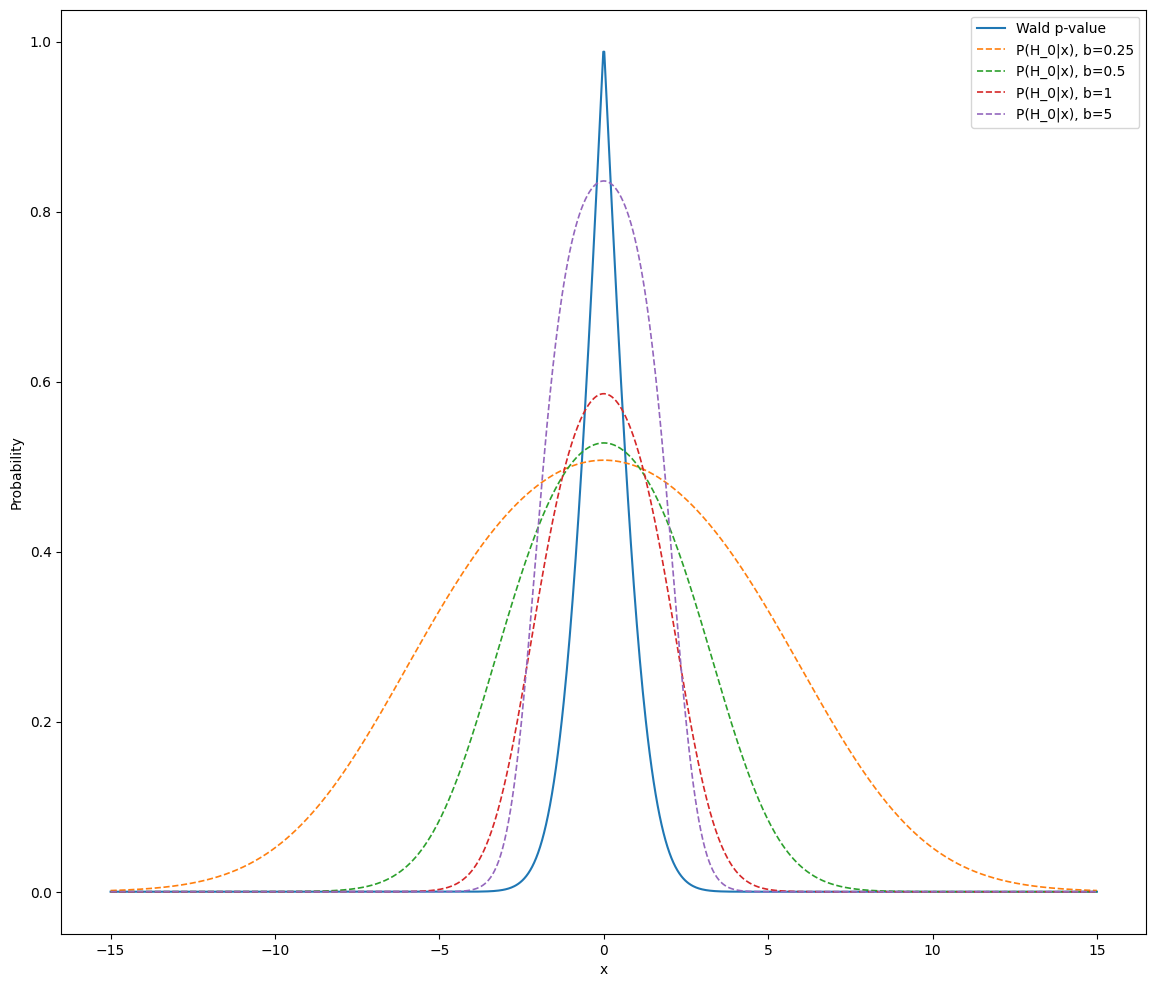
\includegraphics[scale=0.54]{../images/11-08a}
    \caption{Comparison of the posterior probability of $H_0$ for different
      values of $b$ and the Wald test $p$-value as a function of $x$.}
  \end{figure}

  If instead we have a sample of size $n$,
  \begin{align*}
     & \int_{-\infty}^\infty \L(\mu)f(\mu)\,\d\mu                                                                       \\
     & \,=\int_{-\infty}^\infty\prod_{i=1}^n\left[\frac{1}{\sqrt{2\pi}}\exp\left\{-\frac{(x_i-\mu)^2}{2}\right\}\right]
    \frac{1}{\sqrt{2\pi b^2}}\exp\left\{-\frac{\mu^2}{2b^2}\right\}\,\d\mu                                              \\
     & \, =(2\pi)^{-n/2}(b^2n+1)^{-1/2}\exp\left\{-\frac{\beta-\alpha^2/(b^2n+1)}{2}\right\}
    \int_{-\infty}^\infty \frac{\sqrt{b^2n+1}}{\sqrt{2\pi b^2}}\exp\left\{
    -\frac{\left(\mu-\frac{b^2\alpha}{b^2n+1}\right)^2}{2b^2/(b^2n+1)}
    \right\}\,\d{\mu}                                                                                                   \\
     & \, =(2\pi)^{-n/2}(b^2n+1)^{-1/2}\exp\left\{-\frac{\beta(b^2n+1)-\alpha^2}{2(b^2n+1)}\right\},
  \end{align*}
  since
  \begin{align*}
    b^2\sum_{i=1}^n(x_i-\mu)^2+\mu^2
     & =(b^2n+1)\mu^2-2b^2\left(\sum_{i=1}^nx_i\right)\mu+b^2\left(\sum_{i=1}^n x_i^2\right)                                        \\
     & =(b^2n+1)\left(\mu^2-2\frac{b^2\alpha}{b^2n+1}\mu+\frac{b^4\alpha^2}{(bn^2+1)^2} \right)-\frac{b^4\alpha^2}{b^2n+1}+b^2\beta \\
     & =(b^2n+1)\left(\mu-\frac{b^2\alpha}{b^2n+1}\right)^2+b^2\left(\beta-\frac{b^2\alpha^2}{b^2n+1}\right)                        \\
  \end{align*}
  where $\alpha=\sum_{i=1}^n x_i$ and $\beta=\sum_{i=1}^n x_i^2$.

  Therefore,
  \begin{align*}
    \cP{H_0}{X^n=x^n}
     & =\frac{\L(0)}{\L(0)+\int_{-\infty}^\infty \L(\mu)f(\mu)\,\d{\mu}}                        \\
     & =\frac{(2\pi)^{-n/2}\exp\left\{-\frac{1}{2}\beta\right\}}{
      (2\pi)^{-n/2}\exp\left\{-\frac{1}{2}\beta\right\}
      +(2\pi)^{-n/2}(b^2n+1)^{-1/2}\exp\left\{-\frac{\beta (b^2n+1)-b^2\alpha^2}{2(b^2n+1)}\right\}
    }                                                                                           \\
     & =\frac{\sqrt{b^2n+1}}{\sqrt{b^2n+1}+\exp\left\{\frac{b^2\alpha^2}{2(b^2n+1)}\right\}}    \\
     & =\frac{\sqrt{b^2n+1}}{\sqrt{b^2n+1}+\exp\left\{\frac{b^2n^2\Xbar^2}{2(b^2n+1)}\right\}},
  \end{align*}
  while the Wald test $p$-value for a sample of size $n$ is
  \[
    \P{|Z|>\sqrt{n}|\Xbar|}
    =2\Phi\left(-\sqrt{n}|\Xbar|\right).
  \]

  \inputminted{python}{../code/11-08b.py}
  \begin{figure}[H]
    \centering
    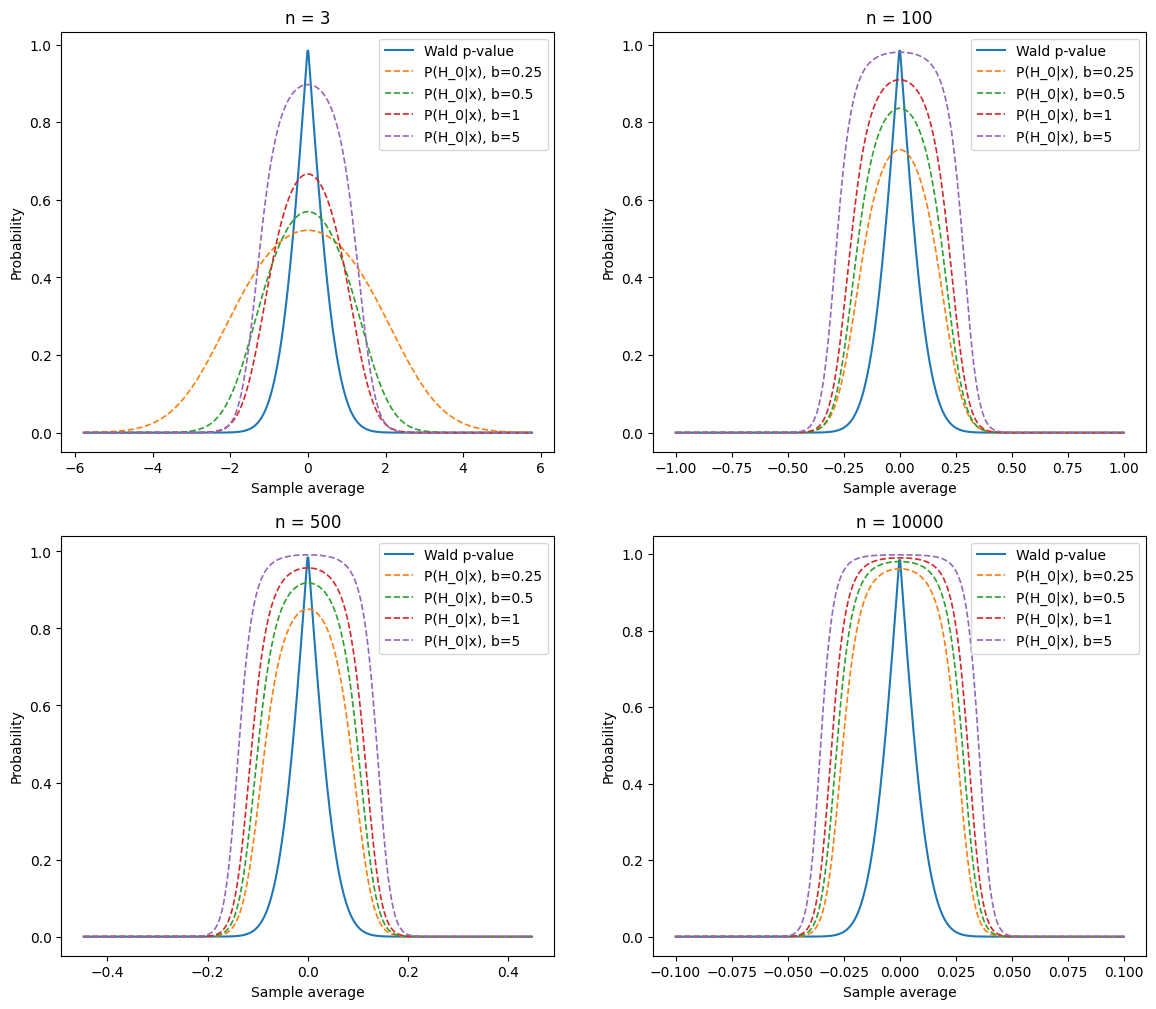
\includegraphics[scale=0.545]{../images/11-08b}
    \caption{Comparison of the posterior probability of $H_0$ for different
      values of $b$ and the Wald test $p$-value as a function of the sample
      average and for different sample sizes. Note that as $n$ increases, a
      region forms in which the $p$-value is near $0$, but the conditional
      probability of $H_0$ is near $1$.}
  \end{figure}

\end{ex}